\chapter{Introduction}

\begin{todo}
	Quelques mots sur le contexte et la problématique
\end{todo}

\section{Jeux de mots}

\subsection{Présentation}

Jeux de mots\footnote{http://jeuxdemots.org} (JDM) est un jeu en
ligne ou les parties des joueurs sont utilisés pour construire un réseau
lexical.

Le déroulement d'une partie est simple.
D'abord une consigne (exemple : \og Donner des idées associés à \fg) et un mot
(exemple : \og parasol \fg) s'affichent.
Le joueur a alors une minute pour proposer ses réponses.
Elles sont ensuite comparées à celles d'un joueur ayant joué cette partie
plus tôt et les mots communs leur rapportent des points.
D'autres mécanismes, comme les \og duels \fg ou les \og procès \fg
incitent les joueurs à jouer plus et ainsi étendre et consolider le réseau.

Un des avantages de l'approche est que le réseau lexical est évolutif, les
parties des joueurs permettent de constantes mises à jour.
De plus, le système étant présenté sous la forme d'un jeu les résultats
obtenus sont plus naturels et représentatifs que ceux fournis pas des 
experts (bien que moins précis).

Au moment de la rédaction de ce document, le réseau de JDM possède 289 873
termes et 4 967 486 relations.

\subsection{Réseau lexical}

Le TALN a besoin de modèles pour représenter l'information lexical et
sémantique, les réseaux lexicaux sont une possibilité.
Un réseau lexical est un graphe dont les sommets sont des termes (mots ou 
expressions) et les arcs sont des relations binaires portant sur le 
lexique ou la sémantique des sommets.
Ces relations sont pondérées afin d'en traduire l'importance.
\citep{lafourcade_tel-00649851}.

\medskip

Dans le réseau lexical de JDM \citep{lafourcade_lirmm-00507777}, on
trouve plusieurs catégories de relation :
\begin{itemize}
	\item relations lexicales : synonymie, antonymie \dots
	\item relations ontologiques : générique (hyperonymie), spécifique
		(hyponymie), partie (méronymie), tout (holonymie).
	\item relations associatives : association libre, sentiment associé,
		signification.
	\item relations prédicatives : agent (sujet), patient (objet),
		instrument \dots
	\item relations de typicalités : lieux, moments, caractéristiques typiques
\end{itemize}

\begin{figure}[!h]
	\centering
	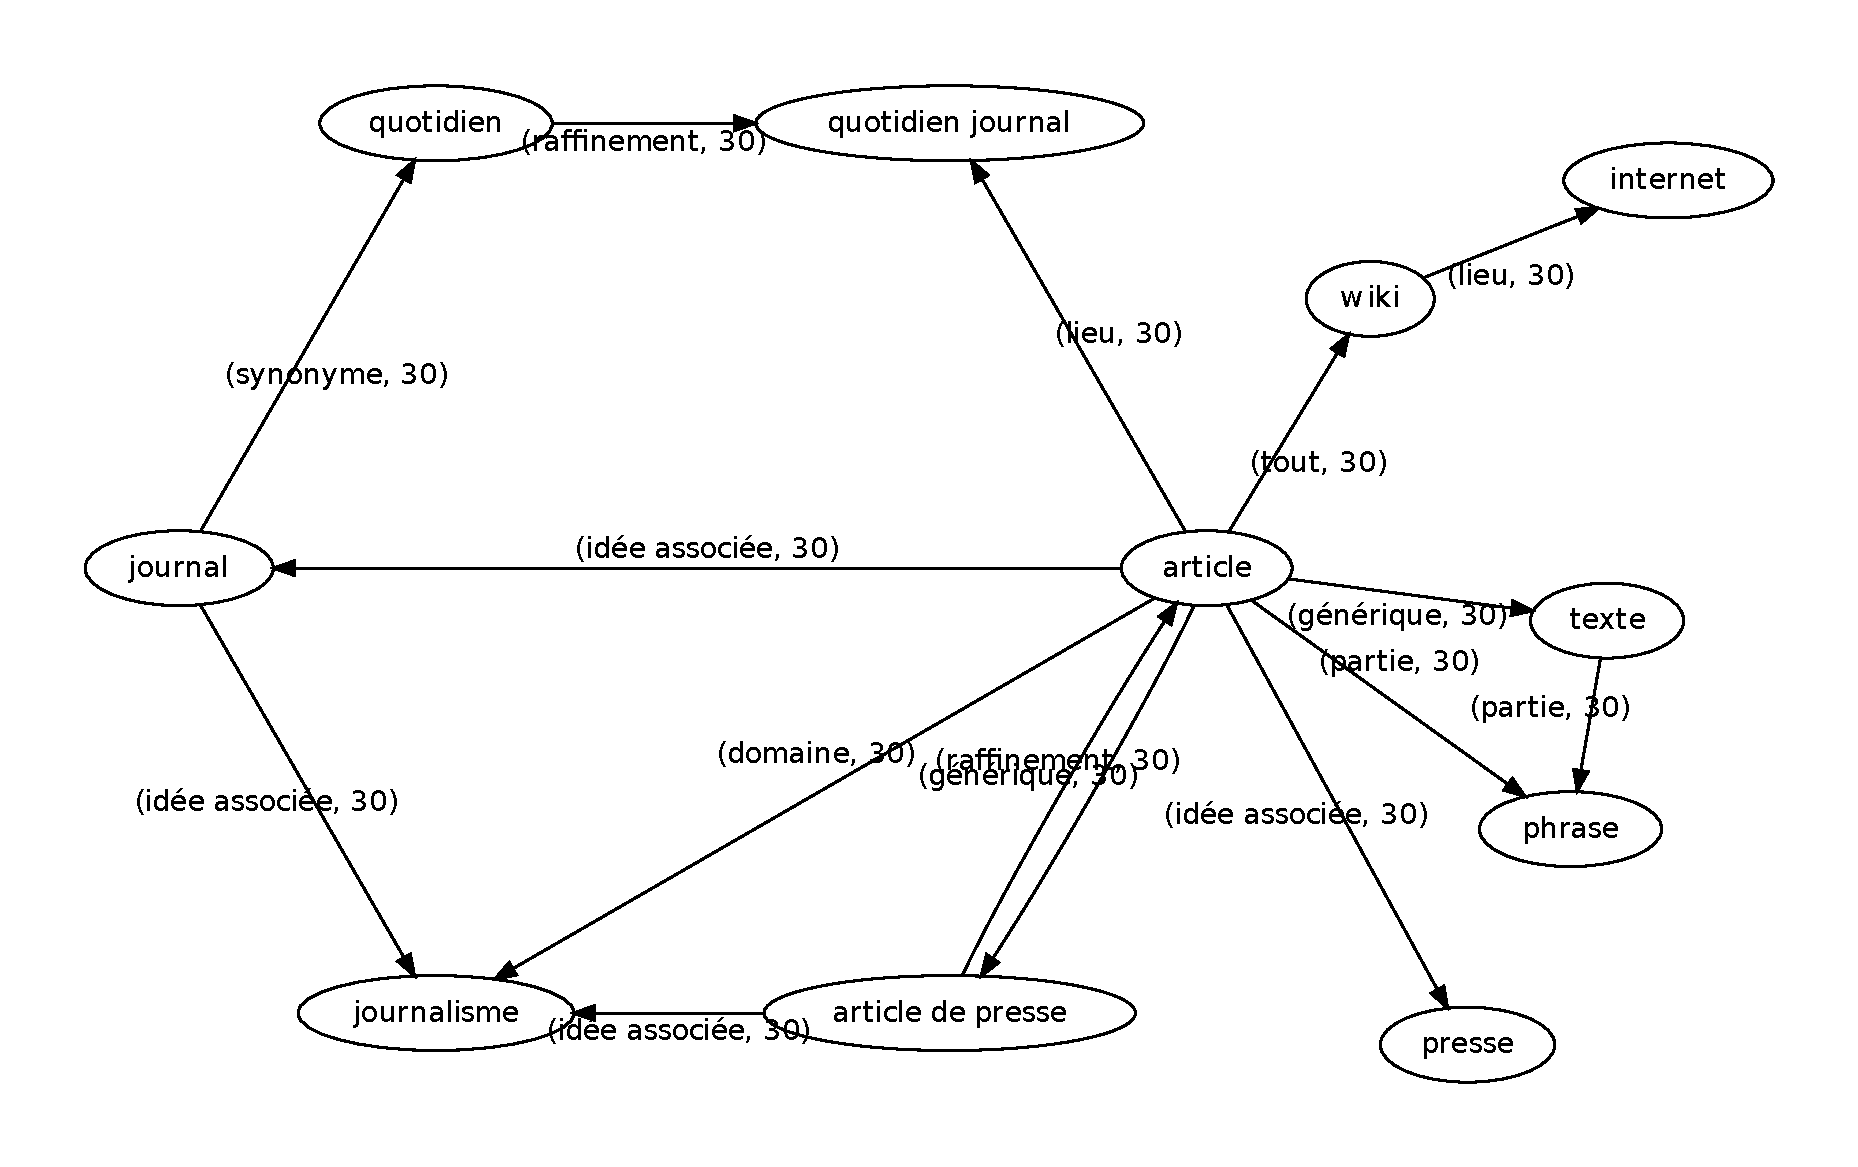
\includegraphics[scale=0.46]{./img/rl1}
	\label{fig:exempleRL1}
	\caption{Exemple de réseau lexical}
\end{figure}

\begin{todo}
	Donner un meilleur exemple, si possible issu de JDM
\end{todo}

On représente un réseau lexical sous la forme d'un graphe orienté :
\begin{align*}
	G &= (V, E) \text{ avec} \\
	&- V : \text{l'ensemble des } n \text{ sommets (mots ou expressions)} \\
	&- E \subseteq V \times V : \text{l'ensemble des } m \text{ arcs (relations lexicales
		ou sémantiques)}
\end{align*}

\subsection{Signature}

Une signature est un ensemble fini et typé de termes pondérés donnant une
définition par extension d'un terme.
Les types sont ceux des relations du réseau et les poids sont la somme 
des poids des relations adjacentes.

Par exemple, la signature du sommet \og article \fg en \ref{fig:exempleRL1}
est :
\begin{align*}
	S(article) = (\text{raffinement} : 34, \text{idée} : 84)
\end{align*}

\begin{todo} ~\\
	Exemple \textbf{réel} \\
	Qu'est-ce que ca représente ? \\
	Notion définissable pour terme, concept, texte entier ... \\
	Différence avec les vecteurs d'idées ? \\
\end{todo}

\section{TOTAKI}

\subsection{Présentation}

TOTAKI\footnote{http://www.jeuxdemots.org/AKI2.php} (Tip of the Tongue and
Automated Knowledge Inferer) est également un jeu en ligne, il a pour objectif
d'évaluer le réseau lexical de JDM \citep{joubert_lirmm-00832991}.
Le principe est de faire deviner un mot au programme.
Le joueur donne successivement des indices auxquels TOTAKI répond par une
proposition.
La partie s'arrête quand le mot est deviné ou si TOTAKI abandonne et demande
la réponse.
Il est possible de préciser la relation que le terme cherché a avec l'indice
donné.

\medskip

\begin{multicols}{2}[Quelques exemples de parties]
	\paragraph{Exemple 1 :}
	\begin{itemize}
		\item méthode $\Rightarrow$ technique
		\item informatique $\Rightarrow$ algorithme \checkmark
	\end{itemize}
	
	\paragraph{Exemple 2 :}
	\begin{itemize}
		\item \texttt{:loc} lampe $\Rightarrow$ ampoule
		\item \texttt{:couleur} bleu $\Rightarrow$ fil
		\item \texttt{:cause} frotter $\Rightarrow$ génie \checkmark
	\end{itemize}
	
	\paragraph{Exemple 3 :}
	\begin{itemize}
		\item logiciel $\Rightarrow$ ordinateur
		\item messagerie $\Rightarrow$ MSN
		\item canaux $\Rightarrow$ client de messagerie
		\item protocole $\Rightarrow$ informatique
		\item chat $\Rightarrow$ \XBox
	\end{itemize}
	Réponse : IRC
\end{multicols}

\subsection{L'algorithme}
\label{sec:revueAlgorithme}

Une fois le premier indice $i_{1}$ donné, on commence par calculer sa
signature $S(i_{1})$ dont les termes sont triés par activations décroissantes.
Le terme le plus activé, noté $max(S)$, est proposé comme réponse $R_{1}$
après avoir retiré l'indice de la signature.
Il est lui même retiré à son tour pour obtenir la signature courante $S'_{1}$ :
\begin{align}
	\begin{split}
		&S(i_{1}) = S_{1} = t_{1}, t_{2}, \dots \\
		&S'_{1} = S_{1} \setminus i_{1} \setminus t_{1} \\
		&R_{1} = max(S_{n}) = t_{1}
	\end{split}
	\label{eq:al1}
\end{align}
Pour tout autre indice $i_{n>1}$, on fait l'intersection entre la signature
courante et celle de $i_{n}$ :
\begin{align}
	\begin{split}
		S_{n} &= (S'_{n-1} \cap S(i_{n})) \setminus i_{n} \\
		S'_{n} &= S_{n} \setminus max(S_{n}) \\
		R_{n} &= max(S_{n})
	\end{split}
	\label{eq:al2}
\end{align}

A chaque itération, le nombre de termes de la signature courante diminue et
termine par être vide si aucune réponse n'est correcte.
Ce stade atteint, le système peut demander la réponse à l'utilisateur ou 
tenter un rattrapage.
La procédure de rattrapage ne se base plus sur l'intersection de signatures,
mais sur leur somme :
\begin{align}
	\begin{split}
		S_{n} &= (S'_{n+1} \oplus S(i_{n})) \setminus i_t \\
		S'_{n} &= S_{n} \setminus max(S_{n}) \\
		R_{n} &= max(S_{n})
	\end{split}
\end{align}

\begin{todo} ~\\
	Décrire la différence intersection / somme \\
	Préciser que le nombre d'application de la procédure doit être limitée
\end{todo}

\section{Problématique}

\begin{todo}

\end{todo}

